\exo7id{6983}
\titre{Exercice 6983}
\theme{}
\auteur{blanc-centi}
\date{2015/07/04}
\organisation{exo7}
\contenu{
  \texte{\'Etudier et tracer les courbes paramétrées suivantes:}
\begin{enumerate}
  \item \question{$\displaystyle\left\{\begin{array}{l}x(t)=\cos^3t\\ y(t)=\sin^3t\end{array}\right.$ {\it (L'astro\"ide)}}
  \item \question{$\displaystyle\left\{\begin{array}{l}x(t)=t-\tanh t\\ y(t)=\frac{1}{\ch t}\end{array}\right.$}
  \item \question{$\displaystyle\left\{\begin{array}{l}x(t)=t-\sin t\\ y(t)=1-\cos t\end{array}\right.$ {\it(La cyclo\"ide)}}
\end{enumerate}
\begin{enumerate}
  \item \reponse{Les expressions $x(t)=\cos^3t$ et $y(t)=\sin^3t$ sont bien définies pour tout $t\in\R$.
\begin{itemize}}
  \item \reponse{Réduction de l'intervalle d'étude\\
Les fonctions $x$ et $y$ étant $2\pi$-périodiques, il suffit de restreindre l'étude à un intervalle de longueur $2\pi$ pour obtenir l'intégralité du support de la courbe.\\

La fonction $x$ est paire, la fonction $y$ est impaire: on fait donc l'étude sur $[0;\pi]$, puis la courbe complète sera obtenue par symétrie par rapport à l'axe $(Ox)$.\\

On constate que $x(\pi-t)=-x(t)$ et que $y(\pi-t)=y(t)$, par conséquent les points $M(\frac{\pi}{2}-t)$ et $M(\frac{\pi}{2}+t)$ sont symétriques par rapport à l'axe $(Oy)$: on restreint donc l'étude à $[0;\frac{\pi}{2}]$, puis on complète par symétrie par rapport à $(Oy)$.\\
\fbox{Finalement, on fait l'étude sur $[0;\frac{\pi}{2}]$} puis on complète
en utilisant successivement les symétries par rapport à $(Oy)$ et $(Ox)$.}
  \item \reponse{Tableau de variations conjointes\\
Les fonctions $x$ et $y$ sont de classe $\mathcal{C}^1$. Soit $t\in[0;\frac{\pi}{2}]$:
$$\begin{array}{lcl}
x(t)=\cos^3t&\ &y(t)=\sin^3t\\
x'(t)=-3\sin t\cos^2t&\ &y'(t)=3\cos t\sin^2t\\
x'(t)<0\Longleftrightarrow t\in]0;\frac{\pi}{2}[&\ &y'(t)>0\Longleftrightarrow t\in]0;\frac{\pi}{2}[\\
x'(t)=0\Longleftrightarrow t\in\{0;\frac{\pi}{2}\} &\ &y'(t)=0\Longleftrightarrow t\in\{0;\frac{\pi}{2}\}
\end{array}$$
$$\begin{array}{c|lcr}
t&0&\ &\frac{\pi}{2}\\\hline
x'(t)&0&-&0\\\hline
\ &1 &\ &\ \\
x&\ &\searrow &\ \\
\ & &\ &0 \\\hline
\ &\ &\ &1 \\
y&\ &\nearrow &\ \\
\ &0 &\ & \\\hline
y'(t)&0&+&0\\
\end{array}$$

Cela signifie que lorsque $t$ varie de $0$ à $\frac\pi2$ la courbe va vers la gauche (car $x(t)$ décroît)
en montant (car $y(t)$ croît) du point $(1,0)$ à $(0,1)$.}
  \item \reponse{Points particuliers\\
  \begin{itemize}}
  \item \reponse{$M(\frac\pi6) = \big(\frac{3\sqrt3}{8},\frac18\big) = (0.64\ldots,0.125) $ ; 
    la tangente est dirigée par $\big(x'(\frac\pi6),y'(\frac\pi6)\big) = \big(-\frac98,\frac{3\sqrt3}{8} \big) = (-1.125,0.64\ldots)$.}
  \item \reponse{$M(\frac\pi4) = \big(\frac{\sqrt2}{4},\frac{\sqrt2}{4}\big) = (0.35\ldots,0.35\ldots)$ ; 
    la tangente est dirigée par $\big(x'(\frac\pi4),y'(\frac\pi4)\big) = \big(-\frac{3\sqrt2}{4},\frac{3\sqrt2}{4}\big) = (-1.06\ldots,1.06\ldots)$.}
  \item \reponse{$M(\frac\pi3) =  \big(\frac18,\frac{3\sqrt3}{8}\big) = (0.125,0.64\ldots)$ ;
    la tangente est dirigée par $\big(x'(\frac\pi3),y'(\frac\pi3)\big) = \big(-\frac{3\sqrt3}{8},\frac98\big) = (-0.64\ldots,1.125)$. 
  \end{itemize}}
  \item \reponse{\'Etude des points singuliers\\
Le point $M(t)$ est singulier si $x'(t)=y'(t)=0$, ce qui est le cas dans le domaine d'étude $[0;\frac{\pi}{2}]$ uniquement pour $t=0$ et $t=\frac{\pi}{2}$. Pour déterminer la tangente au point $M(0)$ (de coordonnées cartésiennes $(1,0)$), on étudie la limite en 0 de 
$$\frac{y(t)-y(0)}{x(t)-x(0)}=\frac{\sin^3t}{\cos^3t-1}$$ 
Or $\sin^3t\underset{0}{\sim}t^3$ et $\cos^3t-1=(1-\frac{t^2}{2}+o(t^2))^3-1\underset{0}{\sim}-3\frac{t^2}{2}$, donc le quotient est équivalent à $-\frac{2}{3}t$ et tend vers 0 en 0. Ainsi, $\mathcal{C}$ admet au point $M(0)$ une tangente, de pente nulle c'est-à-dire horizontale.
\end{itemize}

\begin{center}
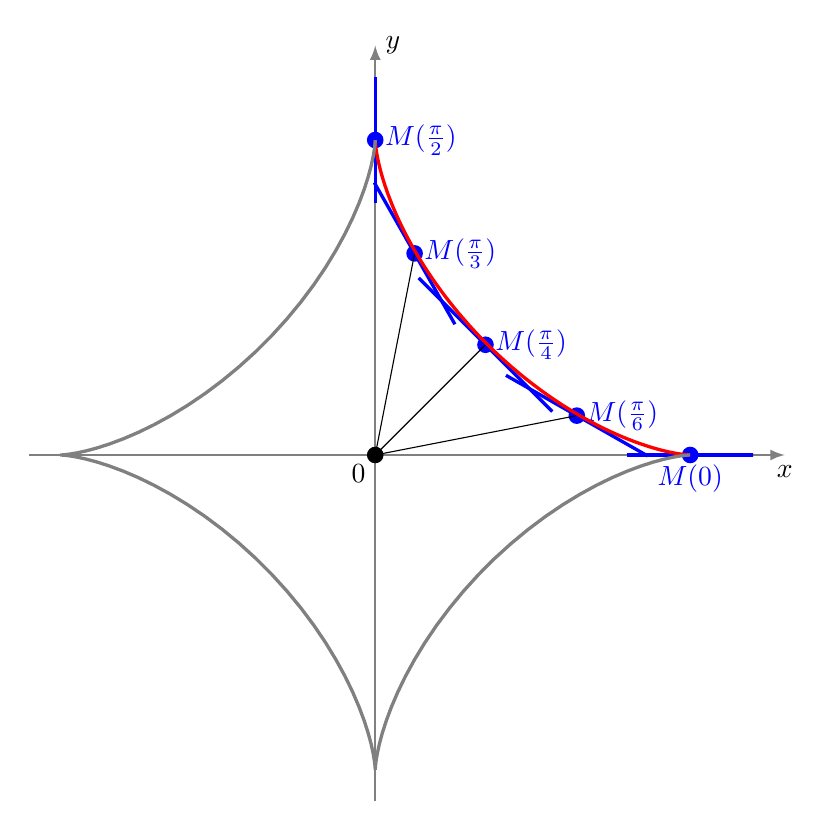
\begin{tikzpicture}[scale=4]
     \draw[->,>=latex,thick, gray] (-1.1,0)--(1.3,0) node[below,black] {$x$};
     \draw[->,>=latex,thick, gray] (0,-1.1)--(0,1.3) node[right,black] {$y$};  



  \fill[black] (0,0) circle (0.75pt) node[below left]{$0$}; 


  \fill[blue] (1,0) circle (0.75pt)  node[below]{$M(0)$}; 
  \fill[blue] (0,1) circle (0.75pt)  node[right]{$M(\frac\pi2)$}; 
  \draw[very thick, blue] (1,0)--+(0.2,0)--+(-0.2,0);
  \draw[very thick, blue] (0,1)--+(0,0.2)--+(0,-0.2);
  
  \def\epsilon{0.2};
  \coordinate (M1) at (0.64,0.125);
  \fill[blue] (M1) circle (0.75pt)  node[right]{$M(\frac\pi6)$}; 
  \draw[very thick, blue] (M1)--+(-\epsilon*1.125,\epsilon*0.64)--+(\epsilon*1.125,-\epsilon*0.64);

  \coordinate (M2) at (0.35,0.35);
  \fill[blue] (M2) circle (0.75pt)  node[right]{$M(\frac\pi4)$}; 
  \draw[very thick, blue] (M2)--+(-\epsilon*1.06,\epsilon*1.06)--+(\epsilon*1.06,-\epsilon*1.06);


    \coordinate (M3) at (0.125,0.64);
  \fill[blue] (M3) circle (0.75pt)  node[right]{$M(\frac\pi3)$}; 
  \draw[very thick, blue] (M3)--+(\epsilon*0.64,-\epsilon*1.125)--+(-\epsilon*0.64,\epsilon*1.125);

  \draw (0,0)--(M1);
  \draw (0,0)--(M2);
  \draw (0,0)--(M3);
  
  \draw[red, very thick,domain=0:pi/2,samples=100] plot ({cos(\x r)^3},{sin(\x r)^3});
  \draw[gray, very thick,domain=pi/2:2*pi,samples=100] plot ({cos(\x r)^3},{sin(\x r)^3});

\end{tikzpicture}  
\end{center}}
  \item \reponse{Les expressions $x(t)=t-\tanh t$ et $y(t)=\frac{1}{\ch t}$ sont bien définies pour tout $t\in\R$.
\begin{itemize}}
  \item \reponse{Réduction du domaine d'étude\\
Comme $x$ est impaire et $y$ paire, \fbox{on restreint l'étude à $\R^+$} puis on complète par symétrie par rapport à l'axe $(Oy)$.}
  \item \reponse{Tableau de variations conjointes\\
Les fonctions $x$ et $y$ sont de classe $\mathcal{C}^1$. Pour $t\in\R^+$:
$$\begin{array}{lcl}
x(t)=t-\tanh t&\ &y(t)=\frac{1}{\ch t}\\
x'(t)=\tanh ^2t&\ &y'(t)=-\frac{\sh t}{\ch ^2t}\\
x'(t)>0\Longleftrightarrow t>0&\ &y'(t)<0\Longleftrightarrow t>0\\
x'(t)=0\Longleftrightarrow t=0 &\ &y'(t)=0\Longleftrightarrow t=0
\end{array}$$
$$\begin{array}{c|lcr}
t&0&\ &+\infty\\\hline
x'(t)&0&+&\ \\\hline
\ &  &\ &+\infty\ \\
x&\ &\nearrow &\ \\
\ &0 &\ & \\\hline
\ &1 &\ & \\
y&\ &\searrow &\ \\
\ & &\ & 0\\\hline
y'(t)&0& - &\ \\
\end{array}$$
Cela signifie que le courbe va vers la droite et vers le bas lorsque $t$ va de $0$ à $+\infty$.}
  \item \reponse{\'Etude des points singuliers\\
Le seul point singulier est $M(0)$, or $\displaystyle \frac{y(t)-y(0)}{x(t)-x(0)}=\frac{1-\ch t}{t\ch t-\mathrm{sh t}}$ et 
$$\frac{1-\ch t}{t\ch t-\mathrm{sh t}}=\frac{-t^2/2+o(t^2)}{t(1+t^2/2+o(t^2))-(t+t^3/6+o(t^3))}\underset{0}{\sim}\frac{-t^2/2}{t^3/3}$$ 
et par conséquent $\frac{y(t)-y(0)}{x(t)-x(0)}\xrightarrow[t\to 0^+]{}-\infty$. Ainsi $\mathcal{C}$ possède une tangente verticale au point $M(0)$ de coordonnées cartésiennes $(0,1)$.}
  \item \reponse{\'Etude des branches infinies\\
Comme $x(t)\xrightarrow[t\to+\infty]{}+\infty$ et $y(t)\xrightarrow[t\to+\infty]{}0$, l'axe des abscisses est asymptote à $\mathcal{C}$.
\end{itemize}

\begin{center}
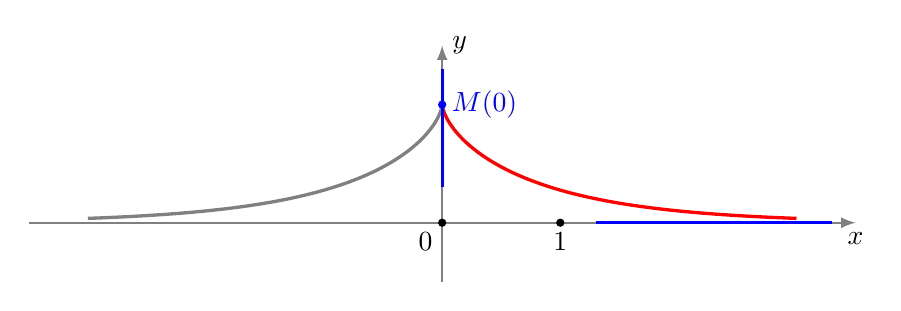
\begin{tikzpicture}[scale=1.5]
     \draw[->,>=latex,thick, gray] (-3.5,0)--(3.5,0) node[below,black] {$x$};
     \draw[->,>=latex,thick, gray] (0,-.5)--(0,1.5) node[right,black] {$y$};  


  \draw[red, very thick,domain=0.2:4,samples=100] plot ({\x - tanh(\x)},{1/cosh(\x)});
  \draw[gray, very thick,domain=-0.2:-4,samples=100] plot ({\x - tanh(\x)},{1/cosh(\x)});

  \fill[black] (0,0) circle (1pt) node[below left]{$0$}; 


  \fill[black] (1,0) circle (1pt)  node[below]{$1$}; 
  
  \fill[blue] (0,1) circle (1pt)  node[right]{$M(0)$}; 
  \draw[very thick, blue] (0,1)--+(0,0.3)--+(0,-0.7);
  \draw[very thick, blue] (2.3,0)--+(1,0)--+(-1,0);
  
 

\end{tikzpicture}  
\end{center}}
  \item \reponse{Les expressions $x(t)=t-\sin t$ et $y(t)=1-\cos t$ sont bien définies pour $t\in\R$.
\begin{itemize}}
  \item \reponse{Réduction du domaine d'étude\\
On remarque que $x(t+2\pi)=2\pi+x(t)$ et $y(t+2\pi)=y(t)$: le point $M(t+2\pi)$ 
se déduit de $M(t)$ par translation de vecteur $2\pi\cdot\vec{i}$. 
Il suffit donc d'étudier la courbe sur l'intervalle $[-\pi;\pi]$.

La fonction $x$ étant impaire et $y$ paire, on restreint l'étude à $[0;\pi]$ 
puis on complète par symétrie par rapport à l'axe $(Oy)$. \\
\fbox{Finalement, on fait l'étude sur $[0;\pi]$} puis on complète
en utilisant successivement la symétrie par rapport à $(Oy)$, puis des translations successives 
de vecteur $2\pi\cdot\vec{i}$.}
  \item \reponse{Tableau de variations conjointes\\
Les fonctions $x$ et $y$ sont de classe $\mathcal{C}^1$. Soit $t\in[0;\pi]$:
$$\begin{array}{lcl}
x(t)=t-\sin t&\ &y(t)=1-\cos t\\
x'(t)=1-\cos t&\ &y'(t)=\sin t\\
x'(t)>0\Longleftrightarrow t>0&\ &y'(t)>0\Longleftrightarrow 0<t<\pi\\
x'(t)=0\Longleftrightarrow t=0 &\ &y'(t)=0\Longleftrightarrow t\in\{0;\pi\}
\end{array}$$
$$\begin{array}{c|lcr}
t&0&\ &\pi\\\hline
x'(t)&0&+&2 \\\hline
\ &  &\ &\pi \\
x&\ &\nearrow &\ \\
\ &0 &\ & \\\hline
\ & &\ & 2\\
y&\ &\nearrow &\ \\
\ &0 &\ & \\\hline
y'(t)&0& + &0\ \\
\end{array}$$
La courbe va vers la droite en montant lorsque $t$ varie de $0$ à $\frac\pi2$.}
  \item \reponse{\'Etude des points singuliers\\
Le point $M(0)$, qui est l'origine, est singulier. Pour étudier l'existence d'une tangente en ce point, on considère
$$\frac{y(t)-y(0)}{x(t)-x(0)}=\frac{1-\cos t}{t-\sin t}\underset{0}{\sim}\frac{t^2/2}{t^3/6}$$
et donc $\frac{y(t)-y(0)}{x(t)-x(0)}\xrightarrow[t\to 0^+]{}+\infty$. Par conséquent, la courbe possède une tangente de pente verticale au point $M(0)$.
\end{itemize}

\begin{center}
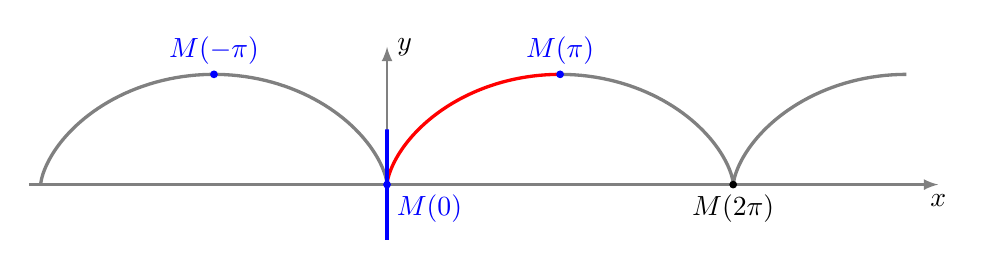
\begin{tikzpicture}[scale=0.7]
     \draw[->,>=latex,thick, gray] (-6.5,0)--(10,0) node[below,black] {$x$};
     \draw[->,>=latex,thick, gray] (0,-.5)--(0,2.5) node[right,black] {$y$};  

  \draw[red, very thick,domain=0:pi,samples=100] plot ({\x - sin(\x r)},{1-cos(\x r)});
  \draw[gray, very thick,domain=pi:3*pi,samples=100] plot ({\x - sin(\x r)},{1-cos(\x r)});
  \draw[gray, very thick,domain=-2*pi:0,samples=100] plot ({\x - sin(\x r)},{1-cos(\x r)});

  \fill[blue] (0,0) circle (2pt)  node[below right]{$M(0)$}; 
  \fill[blue] (3.14,2) circle (2pt)  node[above]{$M(\pi)$}; 
  \fill[black] (6.28,0) circle (2pt)  node[below]{$M(2\pi)$};
  \fill[blue] (-3.14,2) circle (2pt)  node[above]{$M(-\pi)$}; 
  \draw[very thick, blue] (0,0)--+(0,1)--+(0,-1);

\end{tikzpicture}  
\end{center}}
\end{enumerate}
}